\section{Metrics}
\label{sec:Solution} 

%\begin{figure}[H]
	%\centering
		%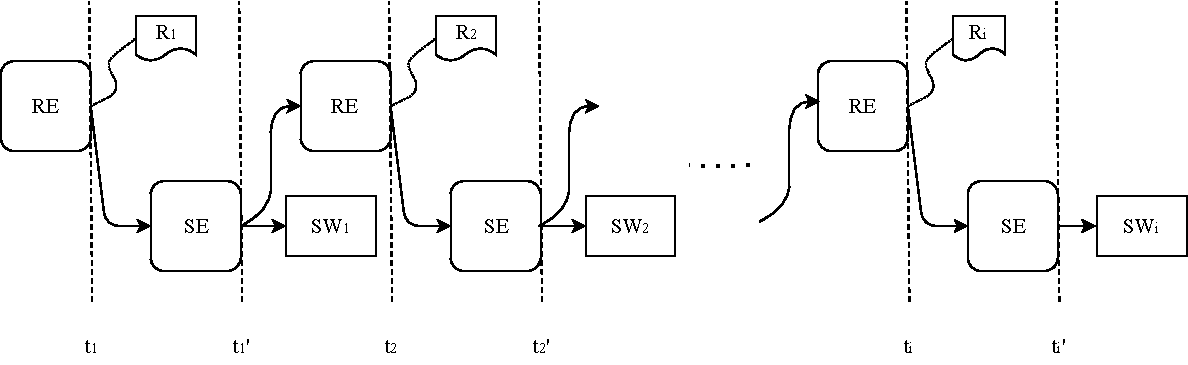
\includegraphics[width=0.8\textwidth,height=2in]{MetricsDiag.pdf}
	%\caption{Requirements engineering and development processes}
	%\label{fig:Metrics_shot}
%\end{figure}

In these metrics we consider a maturity of requirements as a characteristic of the quality.
Every RE artifact (a document with requirements) has its index of maturity. The range of this index varies from 0 to 1: 0 means ``bad'' and 1 indicates ``good'' quality.
The requirements quality presents by a maturity index: coefficient inferred from a number of RE and development process's iterations (a certain amount of changes applied to requirements' document).
The more mature requirements are, the less changes (RE iterations) RE artifact requires in sum, and the shorter time for development process is needed. 

\textsl{thus, the better quality of the requirements; the higher index of the requirements maturity} (\autoref{eqn:maturity_ind}):
  \begin{equation}\label{eqn:maturity_ind}
\textrm{\textit{maturity index}} = \frac{1}{\mu(R_{j})}
	\end{equation}

,where $\mu(R_{j})$ is a calculated number of the iterations for a considered RE artifact $(R_{j}$); $j$ is an initial iteration for calculation.

The input for the first iteration of RE process is a "raw" requirements. During the RE phase, the requirements become elaborated (changed with respect to a project's demands); the result of this process is a corrected RE artifact, that is an input to the next stage (SE). Therefore, we consider the initial RE artifact as a document with a single iteration and \textit{maturity index} = 1. 
\newpage
\hfill \break

\vspace{5.5cm}

\autoref{fig:Metrics_shot} provides a graphical explanation of the metrics. The work flow is divided into RE and SE processes' iterations along the time line: $t_{1},t_{2},...,t_{i}$ - present the time spent for requirements elaboration during RE phases (RE iteration); $t_{1}',t_{2}',...,t_{i}'$ - present the time spent for development process based on the provided requirements (SE iteration).
Output of every RE iteration is a RE artifact (depicted as $R_{1},R_{2},...,R_{i}$ on the); and every SE phase results into a SE artifact, e.g.software architecture (shown as SW), till the end SE phase, which leads to the release of a product and finishing a project.  

Consequently, to calculate the \textit{maturity index} of the requirements, the following metrics should be determined:

 \begin{equation}\label{eqn:mu1}
\mu_{1}(R_{j}) = i-j
	\end{equation}
	
,\textrm{a number of iterations for the requirements} $R_{j}$;

 \begin{equation}\label{eqn:mu2}
\mu_{2}(R_{j}) = t_{i}-t_{j}    
 \end{equation}

,\textrm{amount of time (in hours) between initial and the last phases of RE process applying the requirements} $R_{j}$;

\begin{equation}\label{eqn:mu3}
\mu_{3}(R_{j}) = \displaystyle\sum_{j} t_{j+1}-t_{j}\acute{}
 \end{equation}

,\textrm{total amount of time required for SE process};
%(here, along with requirements' maturity, we can also talk about such quality criterion as the requirements' comprehensibility);

%$\mu_{4} = \displaystyle\sum_{j} (t_{j+1}-t_{j}\acute{} + p_{j}*(t_{j}\acute{} - t_{j}))$
